% !Mode:: "TeX:UTF-8"

\hitsetup{
  %******************************
  % 注意:
  %   1. 配置里面不要出现空行
  %   2. 不需要的配置信息可以删除
  %******************************
  %
  %=====
  % 秘级
  %=====
  statesecrets={公开},
  natclassifiedindex={TP183},
  intclassifiedindex={004},
  %
  %=========
  % 中文信息
  %=========
  ctitleone={局部多孔质气体静压},%本科生封面使用
  ctitletwo={轴承关键技术的研究},%本科生封面使用
  ctitlecover={面向自动驾驶系统测试用例生成的对抗生成网络和图像风格转换技术的实证研究},%放在封面中使用,自由断行
  ctitle={面向自动驾驶系统测试用例生成的对抗生成网络和图像风格转换技术的实证研究},%放在原创性声明中使用
  csubtitle={一条副标题}, %一般情况没有,可以注释掉
  cxueke={工程},
  csubject={计算机技术},
  caffil={南方科技大学},
  cauthor={闫施违},
  csupervisor={张煜群助理教授},
  % 日期自动使用当前时间,若需指定按如下方式修改:
  cdate={2019年6月},
  cstudentid={11749199},
  cstudenttype={同等学力人员}, %非全日制教育申请学位者
  %(同等学力人员)、(工程硕士)、(工商管理硕士)、
  %(高级管理人员工商管理硕士)、(公共管理硕士)、(中职教师)、(高校教师)等
  %
  %
  %=========
  % 英文信息
  %=========
  etitle={An empirical study of GANs and Neural Style Transfers for test case generation in autonomous driving system},
  esubtitle={This is the sub title},
  exueke={Engineering},
  esubject={Computer Technology},
  eaffil={\emultiline[t]{Southern University of Science and Technology}},
  eauthor={Yan Shiwei},
  esupervisor={Prof. Zhang Yuqun},
  % 日期自动生成,若需指定按如下方式修改:
  edate={June, 2019},
  estudenttype={Master of Engineering},
  %
  % 关键词用“英文逗号”分割
  ckeywords={自动驾驶, 深度学习, 对抗生成网络, 图像风格转换},
  ekeywords={autonomous driving, deep learning, GAN, neural style transer},
}

\begin{cabstract}

近年来,得益于深度学习的发展,自动驾驶的研究与开发也取得了巨大的突破。国内外的许多公司都开发了自己的自动驾驶系统框架,譬如Google公司的Waymo,Baidu公司的Apollo和Tesla公司研制的Autopilot,其中最为人熟知的Autopilot已经成功的部署运行在了现实商用的Tesla轿车中。

尽管各大公司都标榜如今的自动驾驶系统安全性能已经足够高,但是近一两年发生的几起自动驾驶车祸引起了人们对于自动驾驶系统安全性能的关注,下左图是于2018年3月23号,发生在美国加州山景城高速公路上的一起车祸,事后事故分析指出由于Autopilot未能识别灰色公路背景下的白色防护栏从而导致的车祸的发生。同样的右图也是由于Uber公司研制的自动驾驶系统的误判,于2017年发生在美国亚利桑那州天普城的一起车祸。

\begin{figure}[h]
  \centering
  \subfigure[车祸1]{
          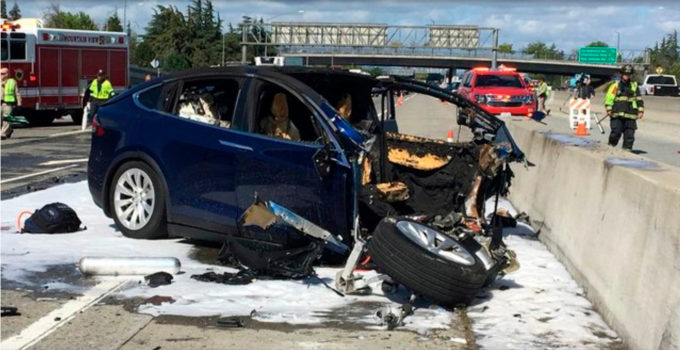
\includegraphics[width=0.45\textwidth, height=4cm]{crash_t}
  }
  \subfigure[车祸2]{
          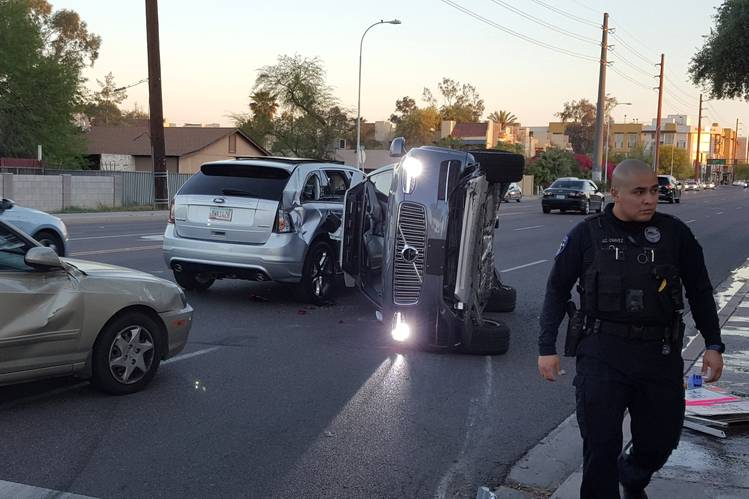
\includegraphics[width=0.45\textwidth, height=4cm]{crash_u}
  }
  \caption{crashes}
\end{figure}

除了上述之外,近年来还陆续有自动驾驶相关的车祸发生,以上种种都表明当前的自动驾驶的安全性能并没有人们认为的那么高。为了提升自动驾驶系统的安全等级,工业界和学术界都在此做了很多研究,于2017年学术界在此领域先后发表了2篇重要的文章,DeepXplore\cite{DeepXplore}和DeepTest\cite{DeepTest},DeepXplore提出了一套深度学习系统测试用例自动生成的框架。DeepTest延伸了DeepXplore的工作并将前者的方法成功的运用到了自动驾驶系统测试用例,即驾驶路况场景图,生成中,两者的工作都以现实的自动驾驶框架为测试对象,成功生成出了很多自动驾驶系统会误判的测试用例,这对提升自动驾驶系统的安全性能有着重大意义。 

基于DeepXplore和DeepTest的工作,DeepRoad\cite{DeepRoad}借助对抗生成网络\cite{GAN}中的UNIT\cite{UNIT}框架提升了生成的自动驾驶测试用例,即驾驶场景图片的质量。在本论文中,我们针对现有的深度学习技术,主要包含对抗生成网络和图像风格转换技术,做了大量的实证研究,以探讨哪些现有的深度学习技术对于自动驾驶测试用例生成,即驾驶场景图片的合成,是最有效的。截止该论文成稿日期,目前学术界还没有针对自动驾驶测试用例生成,即路况图片合成技术的实证研究。 

本工作希望能为之后的自动驾驶系统测试人员在选择驾驶场景图片测试用例自动生成的框架选择上可以给出一些有价值的建议。

\end{cabstract}

\begin{eabstract}
  In recent years, thanks to the development of deep learning, the research and development of autonomous driving has also made great breakthroughs. Many domestic and overseas companies have developed their own autopilot system frameworks, such as Google's Waymo, Baidu's Apollo and Tesla's Autopilot. The most well-known Autopilot has been successfully deployed in real-life commercial Tesla sedan. in.

  Although major companies have advertised that the safety of today's autopilot systems is high enough, several autopilot accidents in the past year or two have caused concern about the safety performance of autopilot systems. The picture on the left is in March 2018. On the 23rd, a car accident occurred on the Highway in Mountain View, California, USA. The post-accident analysis pointed out that the car accident caused the failure of Autopilot to identify the white fence on the gray road background. The same right picture is also due to a misjudgment of the autopilot system developed by Uber, which occurred in 2017 in a car accident in Temple City, Arizona, USA.

  In addition to the above, there have been autopilot-related car accidents in recent years, all of which indicate that the current safety of autonomous driving is not as high as people think. In order to improve the safety level of the automatic driving system, the industry and academia have done a lot of research here. In 2017, the academic community has published two important articles in this field, DeepXplore\cite{DeepXplore} and DeepTest\cite{ DeepTest}, DeepXplore proposes a framework for automatic generation of test cases for deep learning systems. DeepTest extends DeepXplore's work and successfully applies the former method to the autopilot system test case, that is, the driving road scene graph, the generation, both work are based on the actual auto-driving framework as the test object, successfully generated in addition to many automatic Test cases that are misjudged by the driving system are of great significance for improving the safety performance of the autonomous driving system.

  Based on the work of DeepXplore and DeepTest, my lab has proposed DeepRoad\cite{DeepRoad}, which enhances the generated autopilot test case by using the UNIT\cite{UNIT} framework in the anti-generation network \cite{GAN}. The quality of the driving scene picture. In this paper, we have done a lot of empirical research on existing deep learning techniques, including anti-generation network and image style conversion techniques, to explore which existing deep learning techniques are used for autopilot test case generation. That is, the synthesis of the driving scene picture is the most effective.

  This work hopes to give some valuable suggestions for the subsequent autopilot system testers to choose the framework of the auto-generated framework for driving scene picture test cases.
\end{eabstract}

% word count ~ 1000
